%%%%%%%%%%%%%%%%%%%%%%%%%%%%%%%%%%%%%%%%%
% Short Sectioned Assignment LaTeX Template Version 1.0 (5/5/12)
% This template has been downloaded from: http://www.LaTeXTemplates.com
% Original author:  Frits Wenneker (http://www.howtotex.com)
% License: CC BY-NC-SA 3.0 (http://creativecommons.org/licenses/by-nc-sa/3.0/)
%%%%%%%%%%%%%%%%%%%%%%%%%%%%%%%%%%%%%%%%%

%----------------------------------------------------------------------------------------
%	PACKAGES AND OTHER DOCUMENT CONFIGURATIONS
%----------------------------------------------------------------------------------------

\documentclass[paper=a4, fontsize=11pt]{scrartcl} % A4 paper and 11pt font size

% ---- Entrada y salida de texto -----

\usepackage[T1]{fontenc} % Use 8-bit encoding that has 256 glyphs
\usepackage[utf8]{inputenc}
%\usepackage{fourier} % Use the Adobe Utopia font for the document - comment this line to return to the LaTeX default

% ---- Idioma --------

\usepackage[spanish, es-tabla]{babel} % Selecciona el español para palabras introducidas automáticamente, p.ej. "septiembre" en la fecha y especifica que se use la palabra Tabla en vez de Cuadro

% ---- Otros paquetes ----

\usepackage{url} % ,href} %para incluir URLs e hipervínculos dentro del texto (aunque hay que instalar href)
\usepackage{amsmath,amsfonts,amsthm} % Math packages
%\usepackage{graphics,graphicx, floatrow} %para incluir imágenes y notas en las imágenes
\usepackage{graphics,graphicx, float} %para incluir imágenes y colocarlas

% Para hacer tablas comlejas
%\usepackage{multirow}
%\usepackage{threeparttable}

%\usepackage{sectsty} % Allows customizing section commands
%\allsectionsfont{\centering \normalfont\scshape} % Make all sections centered, the default font and small caps

\usepackage{fancyhdr} % Custom headers and footers
\pagestyle{fancyplain} % Makes all pages in the document conform to the custom headers and footers
\fancyhead{} % No page header - if you want one, create it in the same way as the footers below
\fancyfoot[L]{} % Empty left footer
\fancyfoot[C]{} % Empty center footer
\fancyfoot[R]{\thepage} % Page numbering for right footer
\renewcommand{\headrulewidth}{0pt} % Remove header underlines
\renewcommand{\footrulewidth}{0pt} % Remove footer underlines
\setlength{\headheight}{13.6pt} % Customize the height of the header

\numberwithin{equation}{section} % Number equations within sections (i.e. 1.1, 1.2, 2.1, 2.2 instead of 1, 2, 3, 4)
\numberwithin{figure}{section} % Number figures within sections (i.e. 1.1, 1.2, 2.1, 2.2 instead of 1, 2, 3, 4)
\numberwithin{table}{section} % Number tables within sections (i.e. 1.1, 1.2, 2.1, 2.2 instead of 1, 2, 3, 4)

\setlength\parindent{0pt} % Removes all indentation from paragraphs - comment this line for an assignment with lots of text

\newcommand{\horrule}[1]{\rule{\linewidth}{#1}} % Create horizontal rule command with 1 argument of height

\graphicspath{ {./images/} }
\usepackage{subcaption}
\usepackage{hyperref}
\usepackage{soul}


%----------------------------------------------------------------------------------------
%	TÍTULO Y DATOS DEL ALUMNO
%----------------------------------------------------------------------------------------

\title{	
\normalfont \normalsize 
\textsc{\textbf{Aprendizaje Automático (2019)} \\ Doble Grado en Ingeniería Informática y Matemáticas \\ Universidad de Granada} \\ [25pt] % Your university, school and/or department name(s)
\horrule{0.5pt} \\[0.4cm] % Thin top horizontal rule
\huge Memoria Práctica 2 \\ % The assignment title
\horrule{2pt} \\[0.5cm] % Thick bottom horizontal rule
}

\author{Luis Balderas Ruiz \\ \texttt{luisbalderas@correo.ugr.es}} 
 % Nombre y apellidos 


\date{\normalsize\today} % Incluye la fecha actual

%----------------------------------------------------------------------------------------
% DOCUMENTO
%----------------------------------------------------------------------------------------

\begin{document}

\maketitle % Muestra el Título

\newpage %inserta un salto de página

\tableofcontents % para generar el índice de contenidos

\listoffigures

\listoftables

\newpage


%----------------------------------------------------------------------------------------
%	Introducción
%----------------------------------------------------------------------------------------

\section{EJERCICIO SOBRE LA COMPLEJIDAD DE H Y EL RUIDO}

\subsection{Ejercicio 1}

\textbf{Dibujar una gráfica con la nube de puntos de la salida correspondiente:}

\begin{itemize}
	\item[a)] Considere $N=50, dim=2, rango=[-50,50]$ con \textit{simula\_unif}
	
	La ejecución de la función \textit{simula\_unif($50,2,[-50,50]$)} tiene la siguiente salida:
	
	\begin{figure}[H] %con el [H] le obligamos a situar aquí la figura
		\centering
		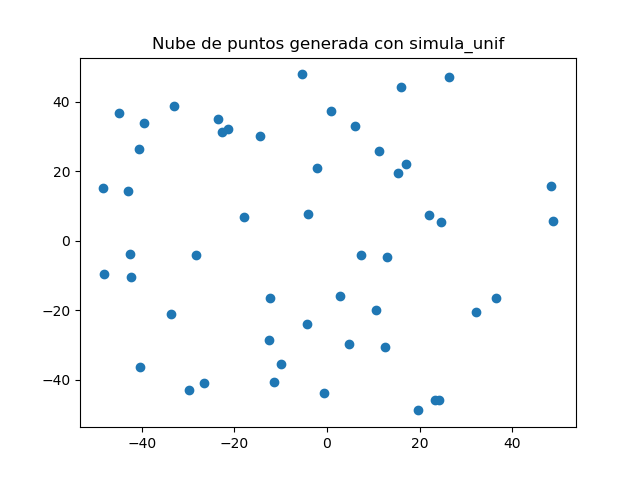
\includegraphics[scale=0.5]{simula_unif1.png}  %el parámetro scale permite agrandar o achicar la imagen. En el nombre de archivo puede especificar directorios
		\caption{Simulación de 50 puntos 2D entre [-50,50] con probabilidad uniforme} 
		\label{fig:simula-unif}
	\end{figure}
	
	\item[b)] Considere $N=50, dim=2, sigma=[5,7]$ con \textit{simula\_gauss}
	La ejecución de la función \textit{simula\_gauss($50,2,[5,7]$)} tiene la siguiente salida:
	
	\begin{figure}[H] %con el [H] le obligamos a situar aquí la figura
		\centering
		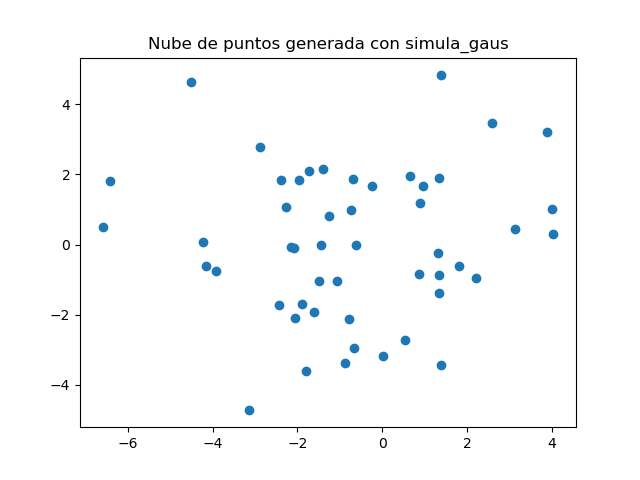
\includegraphics[scale=0.5]{simula_gauss1.png}  %el parámetro scale permite agrandar o achicar la imagen. En el nombre de archivo puede especificar directorios
		\caption{Simulación de 50 puntos 2D de una gaussiana con desviación típica entre [5,7]} 
		\label{fig:simula-gauss}
	\end{figure}
\end{itemize}

\subsection{Ejercicio 2}

\textbf{Con ayuda de la función \textit{simula\_unif()}} generar una muestra de puntos 2D a los que vamos a añadir una etiqueta usando el signo de la función $f(x,y) = y -ax-b$, es decir, el signo de la distancia a cada punto a la recta simulada con \textit{simula\_recta()}

\begin{itemize}
	\item[a)] Dibujar una gráfica donde los puntos muestren el resultado de su etiqueta, junto con la recta usada para ello.
	
	Creo una recta aleatoria con la función \textit{simula\_recta()} de forma que su pendiente y su ordenada en el origen son las siguientes:
	
	$$a = -0.750132431433, b=-14.4754885133$$
	
	Tras generar el dataset de 50 puntos, etiqueto cada uno de ellos en función de si están por encima o por debajo de la recta (cada color indica una situación). El resultado es el siguiente: 
	
	\begin{figure}[H] %con el [H] le obligamos a situar aquí la figura
		\centering
		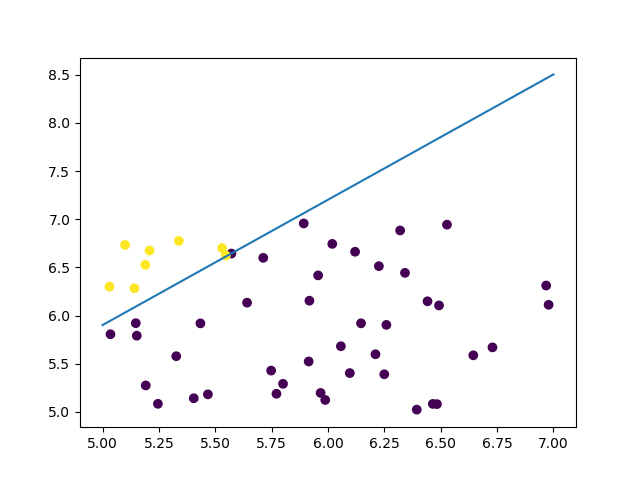
\includegraphics[scale=0.5]{recta1.png}  %el parámetro scale permite agrandar o achicar la imagen. En el nombre de archivo puede especificar directorios
		\caption{Plot de los 50 datos generados uniformemente y la recta aleatoria que los separa en dos partes} 
		\label{fig:recta1}
	\end{figure}

Como se puede ver, todos los puntos están bien clasificados.

	\item[b)] Modifique de forma aleatoria un $10\%$ etiquetas positivas y otro en negativas y guarde los puntos con sus nuevas etiquetas. Dibuje de nuevo la gráfica anterior.
	
	El resultado de esta modificación aleatoria depende mucho de dónde se situó la recta en el apartado anterior. Las dos clases de puntos están desbalanceadas por lo que se verá que una de ellas se cambian menos puntos que la otra. Sin embargo, se garantiza que son el $10\%$ (redondeando a la baja). Veamos el resultado:
	
	\begin{figure}[H] %con el [H] le obligamos a situar aquí la figura
		\centering
		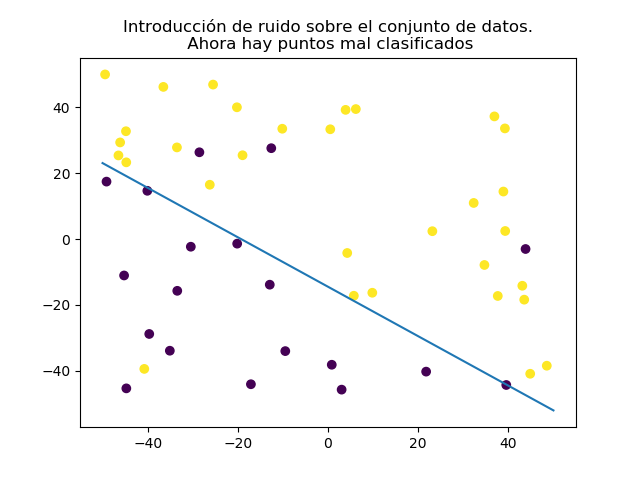
\includegraphics[scale=0.5]{recta2.png}  %el parámetro scale permite agrandar o achicar la imagen. En el nombre de archivo puede especificar directorios
		\caption{Introducción de ruido en el dataset anterior} 
		\label{fig:recta2}
	\end{figure}

Como se puede ver, hay 4 puntos mal clasificados y hemos conseguido que el conjunto no sea linealmente separable.
\end{itemize}

\subsection{Ejercicio 3}

\textbf{Supongamos ahora que las siguientes funciones definen la frontera de clasificación de los puntos de la muestra en lugar de una recta. Visualizar el etiquetado generado en 2b junto con cada una de las gráficas de cada una de las funciones. Comparar las formas de las regiones positivas y negativas de estas nuevas 	funciones con las obtenidas en el caso de la recta ¿Son estas funciones más complejas	mejores clasificadores que la función lineal? ¿En que ganan a la función lineal? Explicar el razonamiento}



\begin{itemize}
	\item $f(x,y) = (x-10)^2+(y-20)^2-400$
	
	\begin{figure}[H] %con el [H] le obligamos a situar aquí la figura
		\centering
		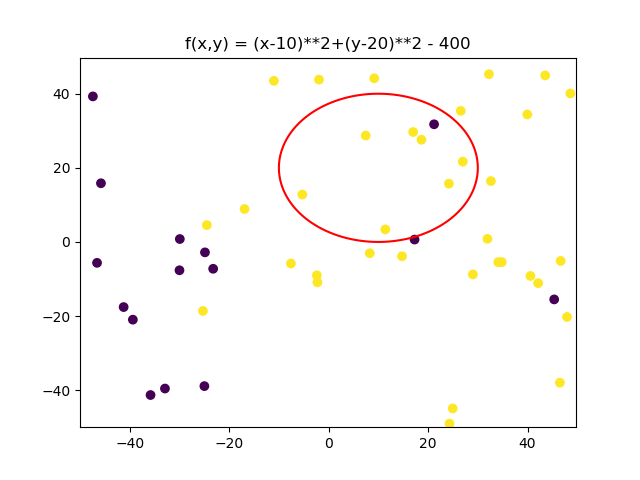
\includegraphics[scale=0.5]{f1.png}  %el parámetro scale permite agrandar o achicar la imagen. En el nombre de archivo puede especificar directorios
		\caption{$f(x,y) = (x-10)^2+(y-20)^2-400$ con los puntos de 2b} 
		\label{fig:f1}
	\end{figure}

Como se puede ver, esta función no sirve para separar las dos clases. La lineal del ejercicio anterior, aunque tiene cuatro errores, separa mucho mejor.

\item $f(x,y) = 0.5(x+10)^2+(y-20)^2-400$
\begin{figure}[H] %con el [H] le obligamos a situar aquí la figura
	\centering
	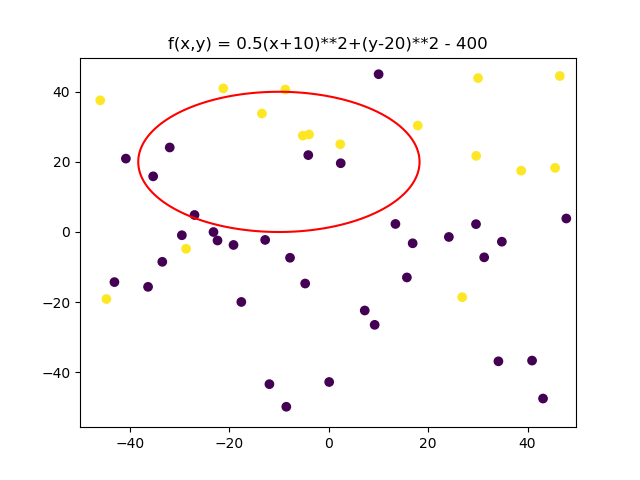
\includegraphics[scale=0.5]{f2.png}  %el parámetro scale permite agrandar o achicar la imagen. En el nombre de archivo puede especificar directorios
	\caption{$f(x,y) = 0.5(x+10)^2+(y-20)^2-400$ con los puntos de 2b} 
	\label{fig:f2}
\end{figure}

De nuevo, se puede ver que no es una función propicia para separar los datos de 2b. No se consigue ninguna ventaja respecto de la recta.

\item $f(x,y) = 0.5(x-10)^2-(y+20)^2-400$
\begin{figure}[H] %con el [H] le obligamos a situar aquí la figura
	\centering
	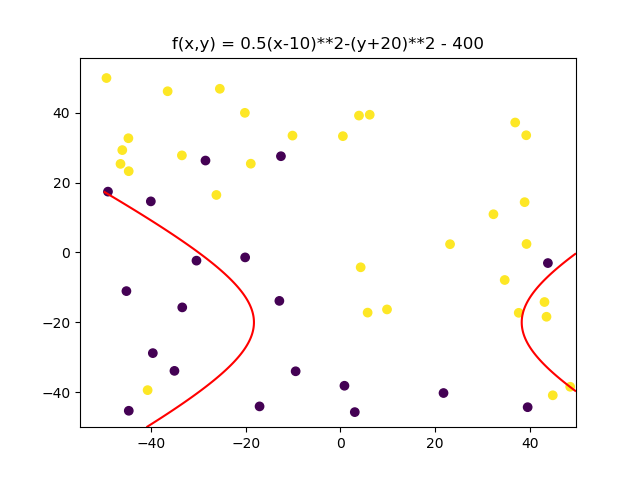
\includegraphics[scale=0.5]{f3.png}  %el parámetro scale permite agrandar o achicar la imagen. En el nombre de archivo puede especificar directorios
	\caption{$f(x,y) = 0.5(x-10)^2-(y+20)^2-400$ con los puntos de 2b} 
	\label{fig:f3}
\end{figure}

Esta hipérbola consigue dejar a derecha izquierda dos clases distintas pero los puntos que se quedan entre medias de las ramas no tienen ninguna separación. Por tanto, tampoco hay ganancia con respecto a la recta.

\item $f(x,y) =  y -20x^2-5x+3$

En este caso, la parábola es la peor función hasta el momento para separar los datos. Veamos:

\begin{figure}[H] %con el [H] le obligamos a situar aquí la figura
	\centering
	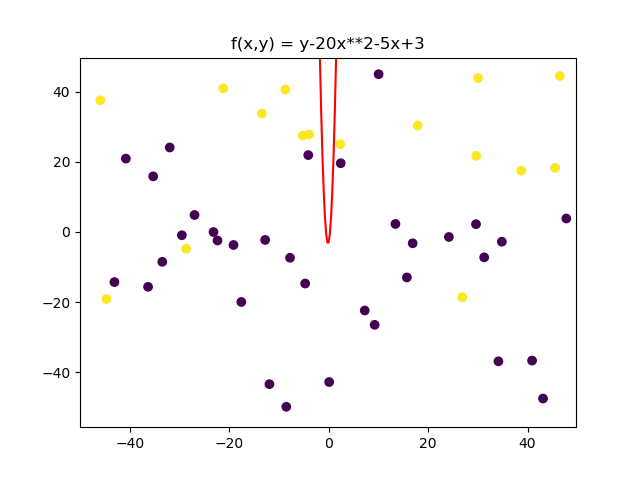
\includegraphics[scale=0.5]{f4.png}  %el parámetro scale permite agrandar o achicar la imagen. En el nombre de archivo puede especificar directorios
	\caption{$f(x,y) =  y -20x^2-5x+3$ con los puntos de 2b} 
	\label{fig:f4}
\end{figure}

Está claro que no genera ningún beneficio en este caso con respecto a la recta.

\end{itemize}

Como se puede ver, ninguna modificación compleja de la función lineal original ha servido para mejorar la clasificación. El motivo es que los datos son prácticamente linealmente separables (solamente han cambiado las etiquetas de 4 puntos) por lo que, a pesar de que no clasificaría el 100\% de los datos bien, comete un error muy pequeño.

\newpage
\section{Bibliografía}

%------------------------------------------------

\bibliography{citas} %archivo citas.bib que contiene las entradas 
\bibliographystyle{plain} % hay varias formas de citar

\end{document}
